\section{Evaluation Methodology}
\label{sec:evaluation-methodology}
\fxfatal{Evaluation Methodology}

In the previous chapter the field of information extraction was presented. The process of IE does not only require the extraction itself, but also the relevance of localized facts for the respective domain. Thus, a quality assessment is required, which focuses on the advancement of development and the juxtaposition of approaches. The evaluation is the formulation of new problems which have to be integrated into the development \cite{Linsmayr:2010}. The methodology of the evaluation is described in this chapter.

\subsection{Performance measures}
A typical way to evaluate an IE system is by using a confusion matrix. This is a well-known
technique of counting results. Figure \ref{tab:confusion-matrix} shows a confusion matrix \cite{Sitter:2004}.

\begin{table}[H]
\centering
\begin{tabular}{cccc}
	& \multicolumn{2}{c}{\shortstack{\textbf{Actual class} \\ (Observation)}} \\
	\multirow{6}{*}{\shortstack{\textbf{Predicted class} \\ (Expectation)}} & \textbf{\textit{tp}}  & \cellcolor{gray!15} \textbf{\textit{fp}} \\
	& (true positive) & \cellcolor{gray!15} (false positive) \\
	& Correct result & \cellcolor{gray!15} Unexpected result \\
	& \cellcolor{gray!15} \textbf{\textit{fn}} & \textbf{\textit{tn}} \\
	& \cellcolor{gray!15} (false negative) & (true negative) \\
         & \cellcolor{gray!15} Missing result & Correct absence of result
\end{tabular}
\caption{Confusion matrix}
\label{tab:confusion-matrix}
\end{table}

For each extracted entity, we have to evaluate if it is correct (and thus a true positive) or not (and thus a false positive). The false negative in the matrix is the number of entities that should have been extracted, but haven't. In IE applications, the true negative is usually not used \cite{Sitter:2004}

Another way to calculate performance measures is based on the notation proposed by \citeauthor{Makhoul:1999} \cite{Makhoul:1999}:

\begin{table}[H]
\centering
\begin{tabular*}{\textwidth}{ll}
	\toprule
	\textbf{Symbol} & \textbf{Meaning} \\
	\midrule
	N & total number of slots in the reference \\
	M & total number of slots in the hypothesis \\
	C & number of correct slots \\
	S & number of substitutions (incorrect slots) \\
	D & number of deletions (missing slots or false rejections) \\
	I & number of insertions (spurious slots or false acceptances) \\
	\bottomrule
\end{tabular*}
\end{table}

The most used evaluation measures in \gls{IE} are recall, precision and F-measure. Some additional ones, like Error per response fill and  Slot error rate, were proposed by \cite{Chinchor:1995} and \cite{Makhoul:1999}.

\subsubsection{Precision}
The \textit{precision} (\ensuremath{\pi} or P), also called Sensitivity, is defined as the percentage of correctly retrieved data in the hypothesis \cite{Carstensen:2010}. 

\begin{figure}[H]
\begin{displaymath}
	\pi = \frac{\textit{tp}}{\textit{tp} + \textit{fp}} = \frac{C}{C+S+I}
\end{displaymath}
\caption{Precision formula}
\end{figure}

\subsubsection{Recall}
The \textit{recall} (\ensuremath{\rho} or R), also referred to as the \gls{PPV}, describes the completeness of an extraction, which is determined by the ratio of correctly predicted results to all correct results \cite{Carstensen:2010}.

\begin{figure}[H]
\begin{displaymath}
	\rho = \frac{\textit{tp}}{\textit{tp} + \textit{fn}} = \frac{C}{C+S+D}
\end{displaymath}
\caption{Recall formula}
\end{figure}

Figure \ref{fig:recall-precision} shows a graphical interpretation of precision and recall. The relevant items are to the left of the straight line while the retrieved items are within the oval. The red regions represent errors. On the left these are the relevant items not retrieved (false negatives), while on the right they are the retrieved items that are not relevant (false positives). Precision and recall are the quotient of the left green region by respectively the oval (horizontal arrow) and the left region (diagonal arrow) \cite{Wikipedia:Precision_and_recall}.

\begin{figure}[H]
\centering
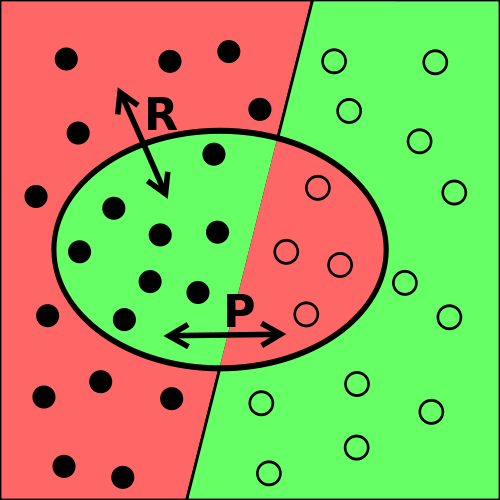
\includegraphics[width=0.35\textwidth]{recall-precision.png}
\caption{Recall and precision example figure \cite{Wikipedia:Precision_and_recall}}
\label{fig:recall-precision}
\end{figure}

\subsubsection{F-measure}
The \textit{F-measure} (F), or  balanced F-score or $\textit{F}_\textit{1}$ score, was introduced to combine \textit{precision} and \textit{recall} into a single measure.

\begin{figure}[H]
\begin{displaymath}
	F_1 = 2 \cdot \frac{\pi \cdot \rho}{\pi + \rho} = \frac{2 \cdot C}{N + M}
\end{displaymath}
\caption{F-measure formula}
\end{figure}

Figure \ref{fig:fbeta-score} shows the more general formula of $\textit{F}_\beta$-score, which contains a parameter $\beta$ to control the balance between \textit{precision} and \textit{recall}. When $\beta$ = 1, $\textit{F}_\textit{1}$ comes to be equivalent to the harmonic mean of $\pi$ and $\rho$. If $\beta$ > 1, F becomes more recall-oriented and if $\beta$ < 1, it becomes more precisionoriented \cite{Sasaki:2007}.

\begin{figure}[H]
\begin{displaymath}
	F_\beta = (1+\beta^2) \cdot \frac{\pi \cdot \rho}{(\beta^2 \cdot \pi) + \rho}, (0 \le \beta \le +\infty)
\end{displaymath}
\caption{$\textit{F}_\beta$-score formula \cite{Chinchor:1992}}
\label{fig:fbeta-score}
\end{figure}

$\textit{F}_\beta$ measures the effectiveness of retrieval with respect to a user who attaches $\beta$ times as much importance to recall as precision \cite{Rijsbergen:1979}.

Another commonly used formula for the F-measure is shown in \ref{fig:falpha-score}. In contrast to Rijsbergen's formula, the balance parameter $\alpha$ is balanced when it's set to 0.5.

\begin{figure}[H]
\begin{displaymath}
	F_\alpha = \frac{\pi \cdot \rho}{(1-\alpha) \cdot \pi + \alpha \cdot \rho}, (0 \le \alpha \le 1)
\end{displaymath}
\caption{$\textit{F}_\alpha$-score formula \cite{Makhoul:1999}}
\label{fig:falpha-score}
\end{figure}

\subsubsection{Accuracy}
\fxfatal{Accuarcy}

\subsubsection{Error measure}
Since \textit{F} is a figure of merit, the higher its value the better we consider the performance of the system. We can then define \textit{E} = 1 – $F_\alpha$ as a corresponding \textit{error measure} \cite{Makhoul:1999}:

\begin{figure}[H]
\begin{displaymath}
	E = 1 - F_\alpha = \frac{S + (1-\alpha) \cdot D + \alpha \cdot I}{(1-\alpha) \cdot N + \alpha \cdot M}, (0 \le \alpha \le 1)
\end{displaymath}
\caption{Error measure formula}
\end{figure}

\subsubsection{Error per Response Fill}
The \textit{Error per Response Fill} (\textit{ERR}) is based on the Error measure and removes the deweighting of \textit{D} and \textit{I} by simply removing the $\alpha$ weights \cite{Chinchor:1995}\cite{Makhoul:1999}.

\begin{figure}[H]
\begin{displaymath}
	\textit{ERR} = \frac{S+D+I}{C+S+D+I}
\end{displaymath}
\caption{Error per response fill formula}
\end{figure}

\subsubsection{Slot Error Rate}
The \textit{Slot Error Rate} (SER) was originally proposed by \citeauthor{Makhoul:1999} \cite{Makhoul:1999} and is basically the Error per response fill metric without the \textit{I} insertion errors in the denominator:

\begin{figure}[H]
\begin{displaymath}
	SER = \frac{S+D+I}{N} = \frac{S+D+I}{C+S+D}
\end{displaymath}
\caption{Slot Error Rate formula}
\end{figure}

\subsection{Discussion}
Often only the F-measure is reported as the evaluation measure of an IE system. If the same weighting for recall and precision is used in calculating the F-measure, this gives an indication of which system is the better one. However, often it may be important to know the individual recall and precision scores of a system to be able to fully compare different systems. When one system has a recall of 10\% and a precision of 90\%, this will obtain the same F-measure as a system which obtains a recall of 90\% and a precision of 10\%, even though both systems are very different. Differences on how a system scores with regards to recall and precision will be unnoticed when reporting only F-measure \cite{Sitter:2004}.

\newpage
\subsection{Runtime performance measures}

\subsubsection{CPU time}
An important metric to measure the runtime performance of a program is the CPU time which determines how much CPU time a process required during its execution.

\subsubsection{Memory consumption}
